\documentclass{beamer}
\usepackage{listings}
\usetheme{Copenhagen}
\usecolortheme{beaver}
\setbeamertemplate{navigation symbols}{}
\setbeamertemplate{footline}{\parbox[t][12pt][c]{12pt}{~\scriptsize\insertframenumber}}
% \usepackage{beamerthemesplit} // Activate for custom appearance

\title{Declarative Cartography}
\subtitle{In-Database Map Generalization of Spatial Datasets}
\author{Pimin Konstantin Kefaloukos, Marcos Vaz Salles, Martin Zachariasen}
\date{\today}

\begin{document}

\frame{\titlepage}

% MOTIVATION
\frame
{
  \frametitle{Motivation}
  \begin{itemize}
  \item Zoomable map based on vector data (new data daily)
  \item At lower scales: too many objects to fit the map
  \item Map should balance \emph{representation} and  \emph{legibility}~\footnote{This map of tourism POI has only representation, not legibility}
  \item We need \emph{generalization} that is easy!
  \end{itemize}

  \fbox{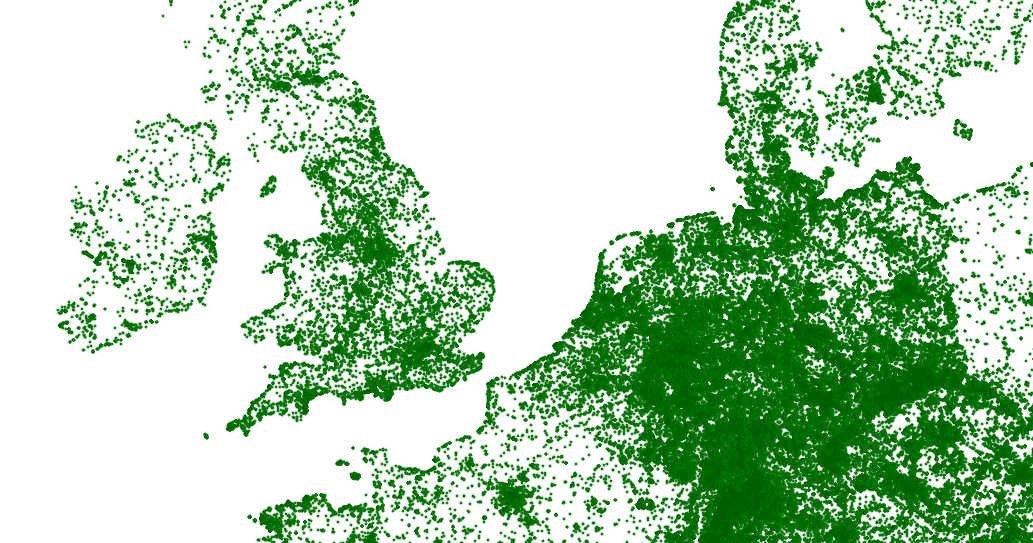
\includegraphics[scale=0.23]{figs/toomanyobjects.png}}
}

\frame
{
  \frametitle{Generalization}
  Two types of generalization:
  \begin{itemize}
  \item Model generalization: Representation in database
  \item Cartographic generalization: Symbolization
  \item \emph{In this work we focus on model generalization}
  \end{itemize}
}

\frame
{
  \frametitle{Operators}
  Examples of operators for model generalization
  \begin{itemize}
  \item Selection
  \item Collapse
  \item Aggregation
  \item Simplification
  \item ...
  \item \emph{In this work we focus on selection}
  \end{itemize}
}

\frame
{
  \frametitle{How we (often) do it today}
  Cartography in practice:
  \begin{itemize}
  \item Styled Layer Descriptor (SLD), Mapnik
  \item Combines selection and cartographic generalization
  \item Selection based on attribute values
  \item Example: \emph{if bycycle path $\rightarrow$ show on $z=\lbrack 20, 11\rbrack$}
  \item Selection is explicit, aesthetic constraints are implicit
  \item \emph{In our work we flip this around}
  \end{itemize}
}

\frame
{
  \frametitle{What if we just have a set of objects?}
 \begin{center}
  	\fbox{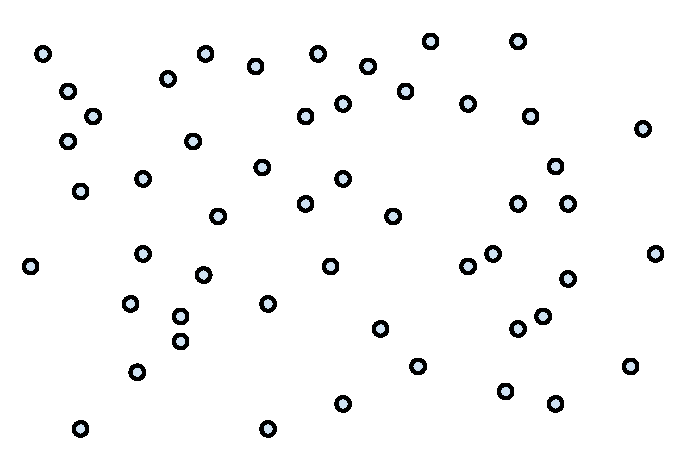
\includegraphics[scale=0.8]{figs/cvl-points.pdf}}
  \end{center}
}


\frame
{
  \frametitle{Conflict sets}
  \emph{Different pieces of information have to '{fight}' for their representation in a specific level of detail - Monika Sester}
  
  \begin{center}
  	\fbox{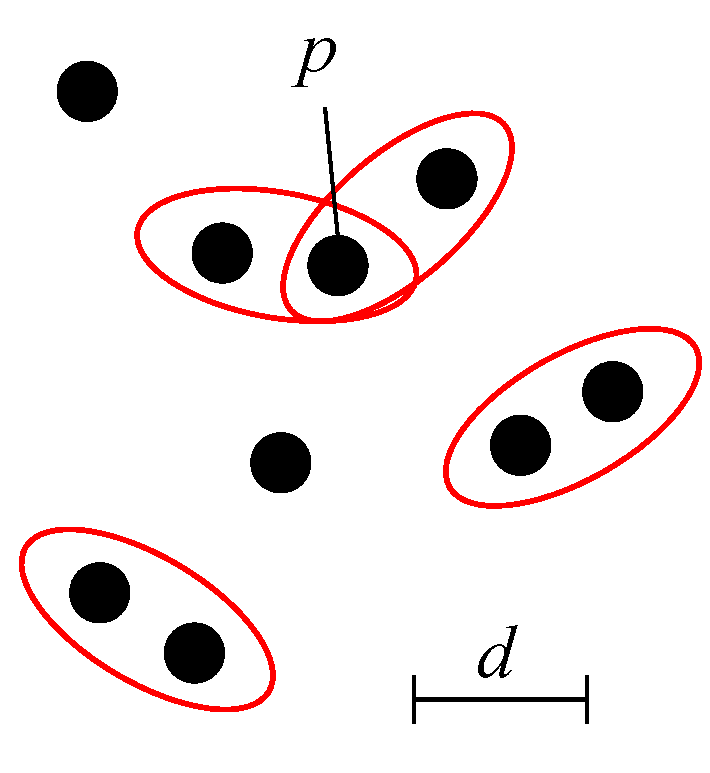
\includegraphics[scale=0.20]{figs/cvl_proximity_conflicts.pdf}} \fbox{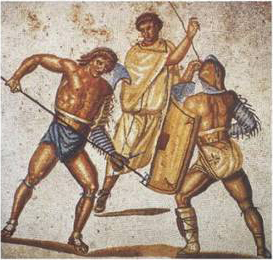
\includegraphics[scale=.38]{figs/gladiators.jpg}}
  \end{center}
  
  \begin{itemize}
  \item A conflict is subset of records, a subset of which have to be eliminated
  \item Conflicts generated by aesthetic constraints
  \end{itemize}
}



\frame
{
  \frametitle{Constraint: Visibility}
  \begin{center}
  	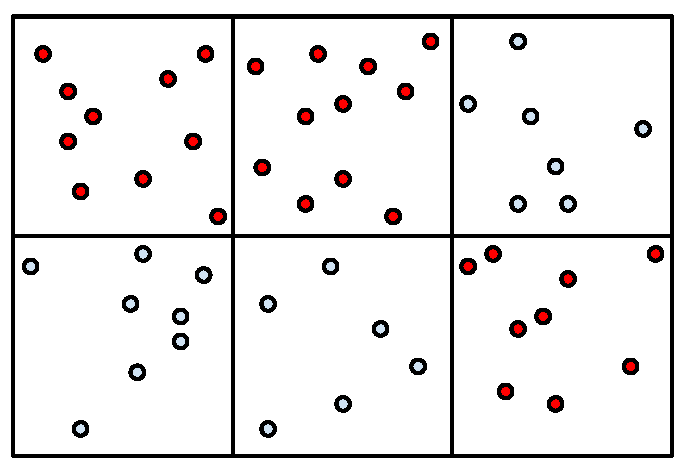
\includegraphics[scale=0.8]{figs/cvl-visibility.pdf}
  \end{center}
  $K=8$
  
 
}

\frame
{
  \frametitle{Constraint: Visibility}
  \begin{center}
  	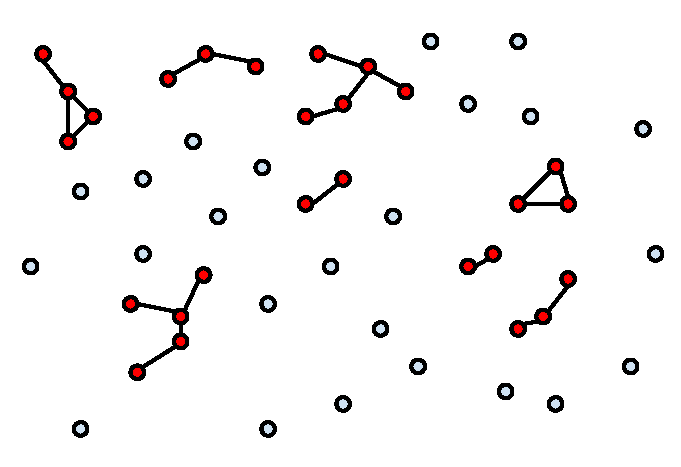
\includegraphics[scale=0.8]{figs/cvl-proximity.pdf}
  \end{center}
 
}

\frame
{
  \frametitle{Problem}
  \begin{itemize}
  \item Assign a \emph{weight} to each object (models importance)
  \item Choose objects on each zoom-level such that constraints are respected + minimize weight that is lost
  \item Further constraint: \emph{Zoom-consistency}
  \end{itemize}
  \begin{center}
  	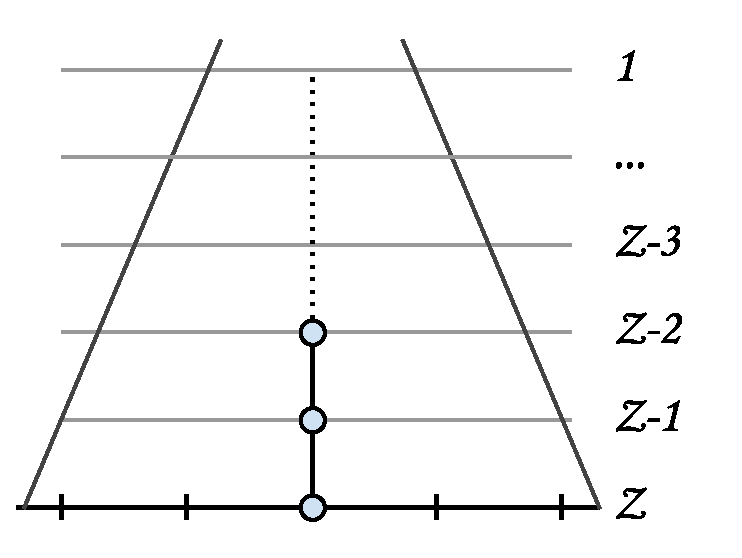
\includegraphics[scale=0.5]{figs/cvl-problem.pdf}
  \end{center}
 
}


% LANGUAGE
\frame
{
  \frametitle{CVL: Cartographic Visualization Language}
  
  \begin{center}
  \fbox{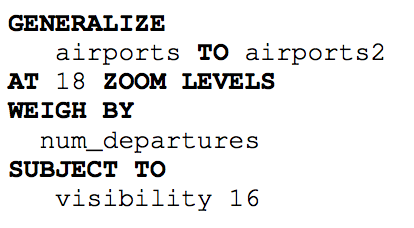
\includegraphics[scale=0.23]{figs/cvlexample.png}}
  \end{center}

  \begin{itemize}
  \item CVL, a language for model generalization (selection)
  \item CVL compiler generates a database program $P$ from CVL
  \item $P$ generates $\mathcal{Z}$ instances of problem 2 (one after the other)
  \item $P$ solves the instances (using database implementation of algorithm for set multicover problem)
  \item Algorithm to use is argument to CVL compiler
  \end{itemize}
}

% DEFINING CONSTRAINTS
\frame
{
  \frametitle{Defining constraints in SQL}
  \fbox{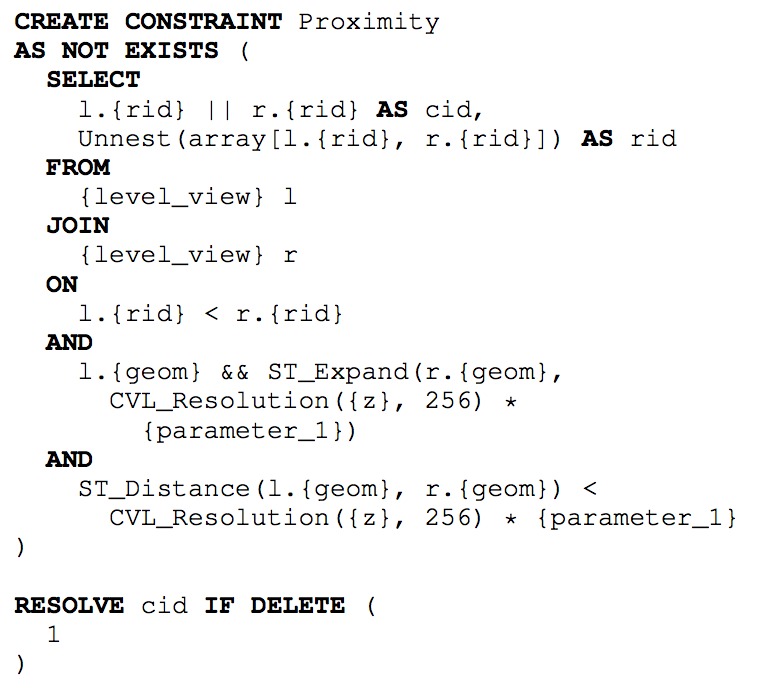
\includegraphics[scale=0.20]{figs/constraintexample.png}}
  \begin{itemize}
  \item Constraints are written in SQL
  \end{itemize}
}

% RELATED WORK
\frame
{
  \frametitle{What does a result look like?}
  The result of running the example CVL script on a database of spatial data:\\
  \fbox{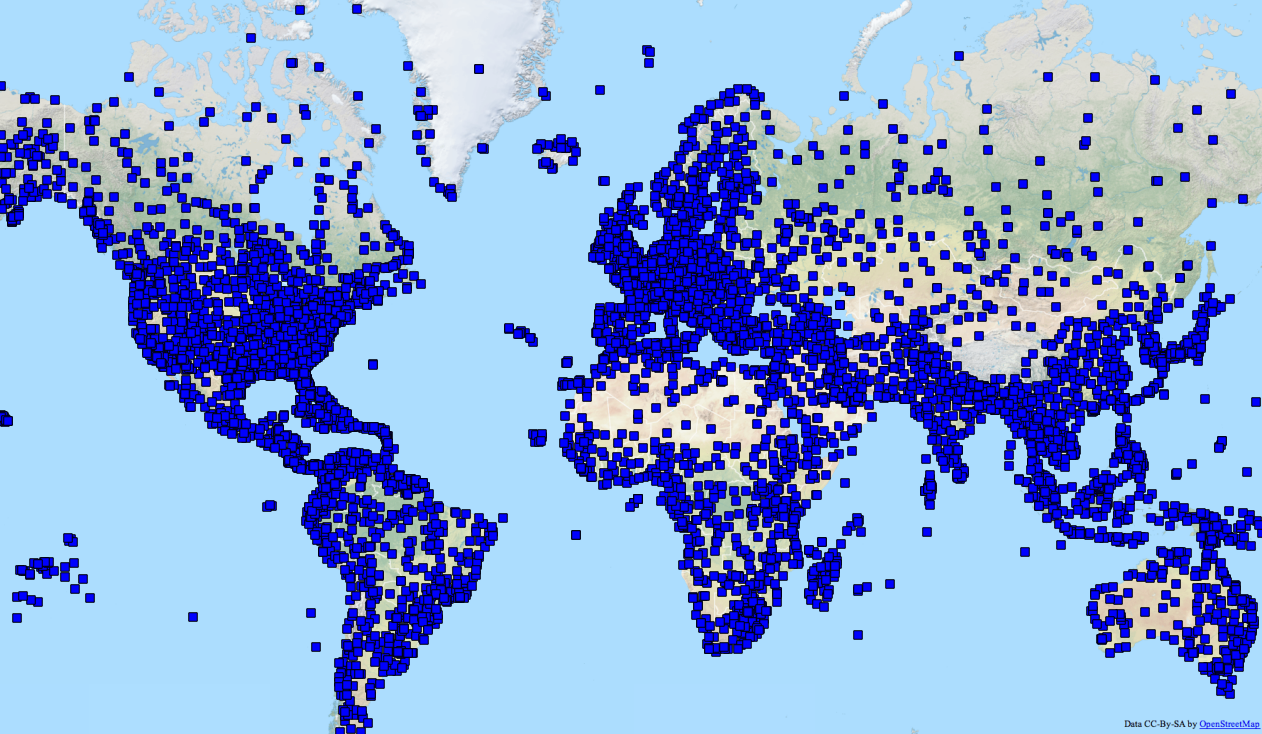
\includegraphics[scale=0.1]{figs/airports.png}}
  \fbox{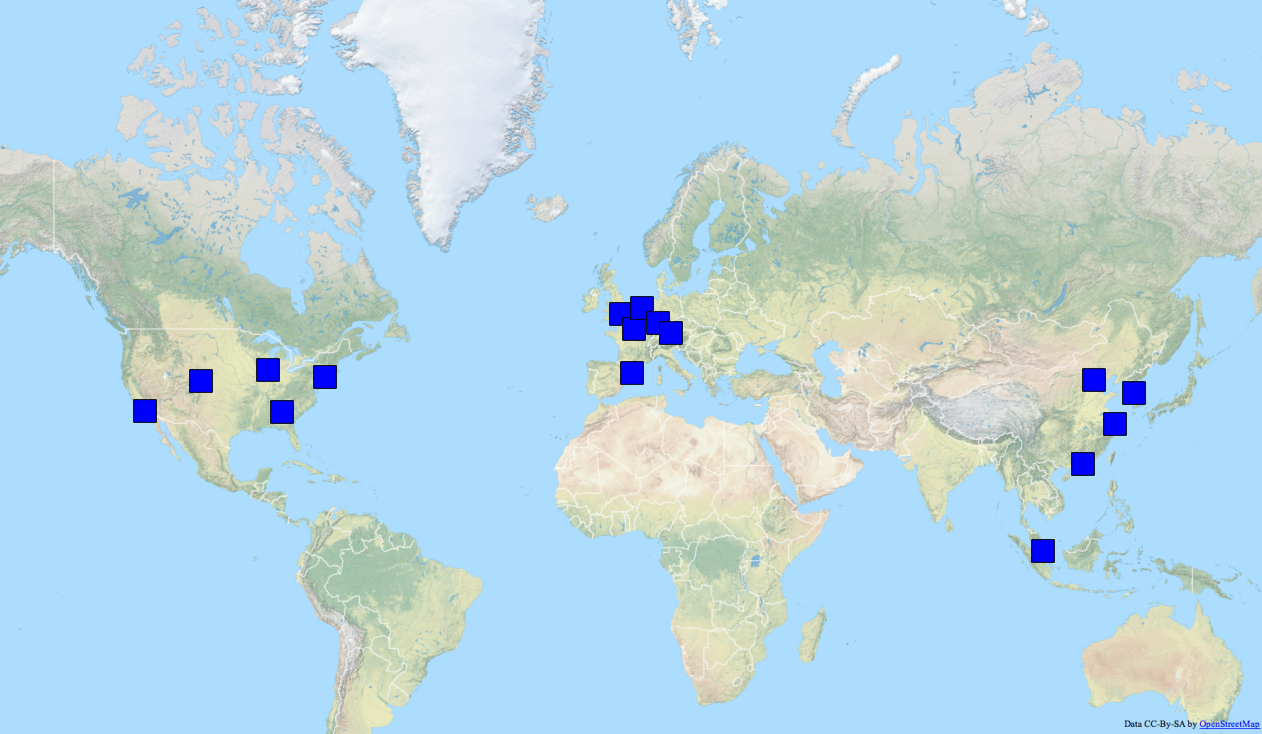
\includegraphics[scale=0.1]{figs/airports_z0.png}}
}


% RELATED WORK
\frame
{
  \frametitle{Related work}

  \begin{itemize}
  \item \emph{Reverse data management}, Meliou, A., Gatterbauer, W., \& Suciu, D. (2011).
  \item \emph{Efficient Spatial Sampling of Large Geographical Tables}. Das Sarma, A., Lee, H., Gonzalez, H., Madhavan, J., \& Halevy, A. (2012).
  \item \emph{Generalization of land cover maps by mixed integer programming}. Haunert, J.-H., \& Wolff, A. (2006). 
  \item \emph{Constant information density in zoomable interfaces}. Woodruff, A., Landay, J., Stonebraker, M. (1998).
  \end{itemize}
}

% Past and future work
\frame
{
  \frametitle{Past and future work}

  \begin{itemize}
  \item Past work: \emph{TileHeat}, predicting where people will look on a map tomorrow
  \item Latest work: \emph{Declarative Cartography}, the work described in these slides
  \item Future work: \emph{Real-time Declarative Cartography}, joint work with people at University of Zurich (Department of Geography)
  \item Future work: Succinct data representation of high-fidelity spatial data that is visualized on a digital map on a screen (think: pixel precision is not all that good)
  \end{itemize}
}




\end{document}
